% Template file for a standard thesis
\documentclass[11pt]{isuthesis}
\usepackage[pdftex]{graphicx}
%\usepackage[utf8]{inputenc}
%\usepackage{float}
%\usepackage{graphicx}
%\usepackage[english]{babel}
\usepackage{amsmath}
\usepackage{float}

% Standard, old-style thesis
\usepackage{isutraditional}   \chaptertitle
\usepackage{comment}

% Old-style, thesis numbering down to subsubsection
\alternate
\usepackage{rotating}


% Bibliography without numbers or labels
\usepackage{natbib}
%\bibliographystyle{apa}


%Optional Package to add PDF bookmarks and hypertext links
\usepackage[pdftex,hypertexnames=false,linktocpage=true]{hyperref}
\hypersetup{
	colorlinks=true,
	linkcolor=blue,
	anchorcolor=blue,
	citecolor=blue,
	filecolor=blue,
	urlcolor=blue,
	bookmarksnumbered=true,
	pdfview=FitB
}

% Use import if there are .tex files called from chapter1.tex (a table for instance) 
\usepackage{import} 

% include path for figures
\graphicspath{{figures/}}

\newenvironment{thesis}{}{}
\excludecomment{thesis} % will exclude material that is only for the thesis


\begin{document}
\DeclareGraphicsExtensions{.jpg,.pdf,.mps,.png}
% Template Titlepage File
\title{Compare RNA-Seq Differential Expression Analysis Methods}

\author{Xiyuan Sun}
\mprof{Jarad Niemi}
\major{Statistics Department}

%--------- MASTER OF SCIENCE -------------
\degree{MASTER OF SCIENCE}
\level{master's}
\members{Jarad Niemi \\ Danniel Nettleton \\ Peng Liu}
%-----------------------------------------
\notice

%-------------  PhD Dissertation -------------------
% Add these additional lines for a Doctoral Dissertation
%\degree{Master of Science}
%\level{master}
\format{dissertation}
\committee{3}


%-----------CREATIVE COMPONENT ------------------------------
% Add these additional lines for a Creative Component
% - also comment out the \maketitle command
%\format{Creative Component}
%\submit{the graduate faculty}
\maketitle

% Optional thesis dedication
\chapter*{DEDICATION}

I would like to dedicate this thesis to ...


% Table of Contents, List of Tables and List of Figures
\pdfbookmark[1]{TABLE OF CONTENTS}{table}
\tableofcontents
\addtocontents{toc}{\def\protect\@chapapp{}} \cleardoublepage \phantomsection
\addcontentsline{toc}{chapter}{LIST OF TABLES}
\listoftables
\cleardoublepage \phantomsection \addcontentsline{toc}{chapter}{LIST OF FIGURES}
\listoffigures
% Comment out the next line if NOT using chaptertitle
\addtocontents{toc}{\def\protect\@chapapp{CHAPTER\ }}



\cleardoublepage \phantomsection This research was built on Niemi et al's approach \citep{niemi2015empirical}. Their research was supported by National Institute of General Medical Sciences (NIGMS) of the National Institutes of Health and joint National Science Foundation / NIGMS Mathematical Biology Program under award number R01GM109458.  
\cleardoublepage \phantomsection  \begin{abstract}

We simulated RNA-Seq count data based on parameters estimated from a maize RNA-Seq dataset \citep{paschold2012complementation}. We comperehensively compared six differential expression (DE) analysis methods (eBayes, edgeR, DESeq2, DESeq, sSeq, and EBSeq) and evaluated their performance by receiver operator characteristic (ROC) curves and areas under the curve (AUC). eBayes tends to give the best performance in terms of AUC. We observed the following patterns: (1) the difference among methods shrinks as proportion of DE genes (pDiff) increases; (2) the number of genes (nGenes) doesn't affect the methods performance in terms of AUC values; (3) all methods perform better when the number of samples increases. Supplementary materials accompanying this paper is on github at https://github.com/xiyuansun/kellycc. 

 \end{abstract}
        



\newpage
\pagenumbering{arabic}

% Introduction of the Thesis Template File
\chapter{OVERVIEW}



\section{Introduction}

Differential expression exists when the expected value of a phenotype differs from the expected phenotypic values of the other variety. Differential expression can occue if the mean phenotype of a variety is greater than the other variety's or less than the other variety's. I refer to the former as high differential expression (HDE) and the latter as low differential expression (LDE). There is differential expression (DE) if and only if either HDE or LDE holds. Ji et al. \cite{ji2014estimation} introduced an approach to assess gene expression heterosis using microarray data under the assumption that these data are continuous. They built a normal hierarchical model for microarray measurements of transcript abundance that allows borrowing of information across genes to estimate means and variances. They introduced an empirical Bayes framework that first estimates model hyperparameters, then estimates the posterior distribution for gene-specific parameters conditional on those hyperparameters, and finally computes heterosis probabilities based on integrals of regions under this posterior. Building on the work of Ji et al. with the normal data model, Niemi et al. \cite{niemi2015empirical}

The focus here is on methods for count-based differential expression (DE) amalyses. Thus, the starting point here is a count table of features-by-samples, such as those from the Paschold project \cite{paschold2012complementation}.

Considerable recent effort has been paid to the discovery of DE features, given a count table; recent comparisons have shown that no method dominates the spectrum of possible situations \cite{soneson2013comparison}\cite{rapaport2013comprehensive}. 

\section{RNA-Seq Count Data}

RNA-Seq is a next generation sequencing procedure of the entire transcriptome by which one can measure the expression of gene expression. The number of reads mapped to a given gene is considered to be the estimate of the expression level of that feature using the technology. The end product of a RNA-seq experiment is a sequence of read counts, typically represented as a matrix with rows representing genes and columns representing samples from two varieties, as in Table \ref{tab:RNA-Seq Data}. In this example, there are $V=2$ varieties, $J_1 = 2$ samples in the first variety, $J_2=2$ samples in the second variety, and $G=10000$ genes. My interest is in the detection of differentially expressed genes among the varieties. 

\begin{table}[H]
\begin{center}
    \begin{tabular}{|c|c|c|c|c|c|}
      \hline
      Gene &Variety1 Sample1 &Variety1 Sample2 &Variety2 Sample1 & Variety2 Sample2 \\
      \hline
      1 & 4 & 1 & 100 & 88 \\
      \hline
      2 & 65 & 48 & 55 & 59 \\
      \hline
      3 & 0 & 1 & 0 & 2\\
      \hline
      ... & ... & ... & ... & ...\\
      \hline
       10000 & 3 & 1 & 1 & 2\\
       \hline
    \end{tabular}
\end{center}
\caption{RNA-Seq Count Data Example}
\label{tab:RNA-Seq Data}
\end{table}

The focus of this report is to provide a comparison of the methods related to the analysis of differential expression for RNA-seq data. In this report, I review statistical methods for detecting differential expression in the RNA-seq data, including the empirical Bayesian method. I summarize the results of a simulation study. I briefly describe some existing open source R and Bioconductor software for testing differential expression for RNA-seq data. I conclude the report with a discussion section. 




\chapter{METHOD}

\section{Introduction}
Put chapter 1 content here. \cite{lorenz2014using}


\section{Lets make a table} 
% latex table generated in R 3.3.0 by xtable 1.8-2 package
% Thu May 18 10:23:23 2017
\begin{table}[ht]
\centering
\begin{tabular}{rrrrr}
  \hline
 & X1 & X2 & X3 & X4 \\ 
  \hline
1 &   9 &   8 &  14 &  13 \\ 
  2 &   7 &  11 &   9 &  11 \\ 
  3 &   8 &   6 &  10 &   9 \\ 
  4 &   6 &  10 &  11 &  16 \\ 
   \hline
\end{tabular}
\caption{some numbers} 
\label{t1}
\end{table}
 

\section{Lets share an historic moment}

Figure \ref{history} is so amazing  that the rest is indeed obvious.

\begin{figure}[h!tb] \centering
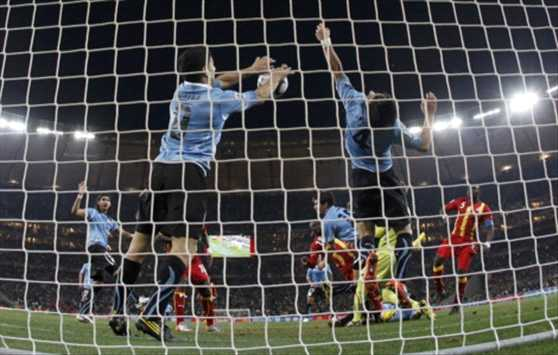
\includegraphics{history}
\caption{Suarez save the day !}
\label{history}
\end{figure}



%\appendixtitle 
%\appendix
%\include{appendix1}
%\include{appendix2}


\renewcommand{\bibname}{\centerline{BIBLIOGRAPHY}}
\unappendixtitle
\newpage
\phantomsection
%\addcontentsline{toc}{chapter}{BIBLIOGRAPHY}
\bibliographystyle{plain}
\bibliography{mybib}

\end{document}
